\documentclass[11 pt,twocolumn,letterpaper]{article}

\usepackage{times}
\usepackage{epsfig}
\usepackage{graphicx}
\usepackage{amsmath}
\usepackage{amssymb}
\usepackage{xcolor}

\usepackage[breaklinks=true,bookmarks=false]{hyperref}

\setcounter{page}{1}
\begin{document}
\begin{titlepage}

\title{Huffman Coding}
\author{Abdallah T.Reda\\
{\tt\small abdallahtamer.ali98@eng-st.cu.edu.eg}
\and
Abdallah M.Shehata\\
{\tt\small abdozza.206@gmail.com(for git) 

 abdallah.mohamad98@eng-st.cu.edu.eg  }
\and
Ezz eldin I.Ezzeldin\\
{\tt\small Ezzeldeen.esmail99@enf-st.cu.edu.eg}
\and
Youssef s.Azmi\\
{\tt\small youssefsamir831999@gmail.com (for git) 

youssef.saleb99@eng-st.cu.edu.eg}
\and
Pola N.kamal\\
{\tt\small pola.gadallah98@eng-st.cu.edu.eg}
}
\maketitle 
\end{titlepage}


\setcounter{page}{2}

\section{Introduction}
    Before we get into our project we need get some points.\\
First of all what is the aim of Huffman. Huffman is a technique  used for encoding \cite{ref1}.\\
It is used to compress the size of files, but how??  \\

It uses the ascii extended table as the following figure \cite{ ASCII}:\\
\begin{figure}[ht]
   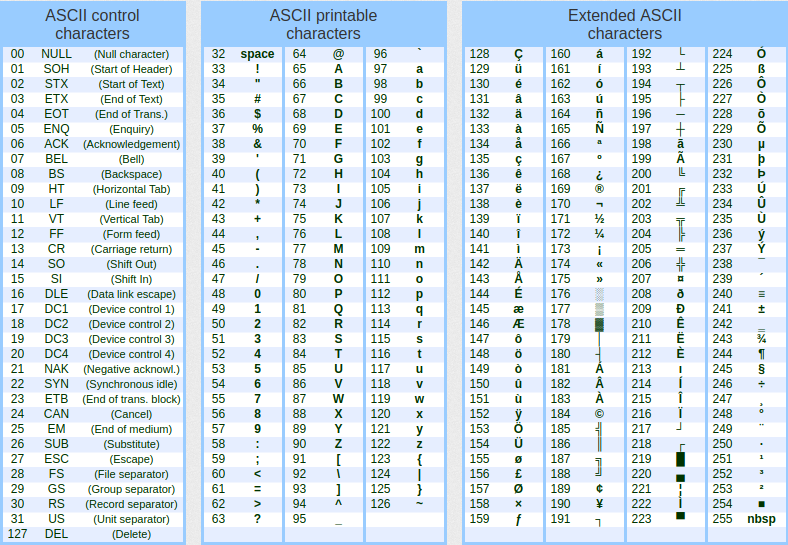
\includegraphics[width=0.8\linewidth]{figure 1}
\end{figure}\\
So that as in our example which is a picture it uses pixels in form of ascii numbers and get the count for each ascii number.\\
It will then form a tree depending on these counters associated with the ascii given. This tree is formed using min heap which was given in sections or we can use priority queue as we used in our project.
After we formed the tree whatever the algorithm we used, we will try to trace this tree or traverse it to get our binary encoded.
The binary depends on the path of the root of the tree. Most of algorithms in google uses 1 for right and 0 for left. But as I remember that in lectures we used the opposite like(anatomical positions),but any way it won’t change the output if we use a single numbering for the whole algorithm.\\
Lets now get closer to our aim. (the pgm pictures).
Pgm refers to portable gray map. It has 2 types, p2 and p5.\cite{PGM}\\
p2 is responsible for storing pixels in ascii, while p5 (which we took in our samples) used to store pixels in binary. Sothat p5 is compressed while p2 is not.
The next picture is a pgm one\cite{PGMB}.
\begin{figure}[ht]
   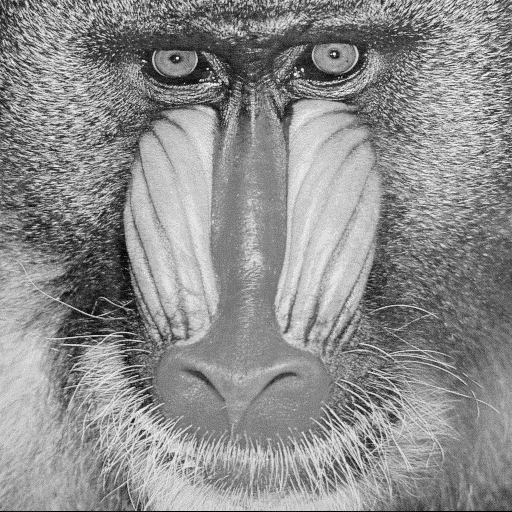
\includegraphics[width=0.8\linewidth]{figure 2}
\end{figure} 
\section{Motivation}
   This project(Huffman encoding) makes us know about a new field which we think it can be an intro to image processing, making a project in this field will help the team members make a good decision if this field is good for them or not.
We searched about the main algorithm of Huffman then we needed to search about types of pictures which made us need to search for types of pgm and how it differs.
So we got a lot of knowledge about many fields such as coding, algorithms, and differentiate between types of image and how to deal with them using different methods.
\section{Resources}
  As we understand from this title we are asked to write the libraries used.
First and main library to use if fstream and sstream, we used them to get inputs or outputs between files and cpp.
We used the command ios::app for example to just copy a text or data from cpp to a file without deleting them, we used also ios::binary to deal with a binary data file such as (p5 pgm).
We used also string and string.h so that we can deal with string through store, print or either know length of string.
Queue also used to make a priority queue that arranges the nodes due to some parameter (which in our case is counters)
there are many other small new commands we used such as vectors , dynamic arrays with 2 dimensions and many others.
\section{Challenges and Problems}
In our project, we met many problems.\\
a)On of the main problems is main idea, at first, the algorithm was difficult to be converted into codes, how to make nodes that merge together forming new nodes and rearrange them and repeat this cycle till having only one node which is the root.
But using the sections videos we get the first idea when we remembered the relation between huffman and min heap so that after period of time we reached another point which is priority queue so the first problem solved.\\
b)The second is the pictures and how to deal with it without using matlab for example, after we made a code to read the picture we found a big problem destroyed our code. Which is pgm has types and we are using another type.
It took about 2 days to know our problem and after many times of trying we made a suitable code for it.\\
c)The last problem was data types. And we are sorry ta say that there is still problem and it until the moment we wrote this report the problem present.
The program is working perfect but the problem is the txt file. The memory stored take a great amount as we store binary data in form of integers. It is the only problem that exist and we are trying hardly to manage.\\
\section{User manual for the system} 
our program is so easy to use just follow the next steps:\\
 Frist thing that a main window will appear and you can choose the operation encode or decode, but please take care of several things:\\
a) make an empty folder that will contain all files that will be made during the running of the program.\\
b) don’t make the same command twice as you will have a problem with overwrite the data, delete the old files first then you can use it again.\\
Now we can get to our 2 conditions which are encoding and decoding:\\
\textcolor{red}{1) in case of encoding:}\\
A) you will be asked to enter picture location in your operating system such as “/home/abdallah/Desktop/data/NORMAL2-IM-1430-0001.pgm”  then you will enter the location for the empty folder that will contain the source, asci ,  encode files.\\
b) enter the names for the files that will be created.\\
c) 3 new files will be created in the location you wrote, which are:\\
i) source file that will store number of cols, rows and max value.\\
ii) asci file that will store the frequency table for the picture.\\
iii)output file that will include the encoded binary for the whole picture.\\
\textcolor{red}{2) in case of decoding:}\\
A) it is similar to encoding, first you will asked to insert the location for the folder containing the ascii, source and output files which are previously made in encoding and the decoded file for returning back the decimal numbers from the binary, and the new image that will be formed with this decoded file which must be the same as the original file to make sure that it is decoded right.\\
B) press on decode button, wait few milliseconds till a message say that the decoded files have been created.\\
c) check your empty file , you will see all previous files were added with the image\\


\section{Results}
First of all we used qmake instead of cmake in the gui version while the terminal using version is with cmake.\\
First thing you will see when you open the program is that window\\
\begin{figure}[ht]
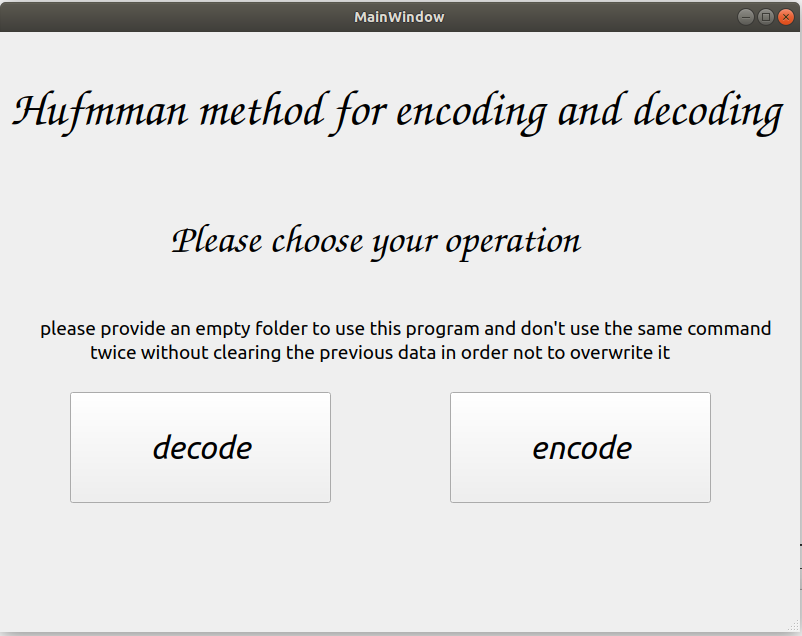
\includegraphics[width=0.8\linewidth]{figure 3}
\end{figure}\\
Lets assume that you clicked the encode button, the next window will appear.\\
This window has simple inputs to get.\\
1) wherever your picture location it doesn’t matter, only copy its location and paste it here.\\
2)make an empty folder then get its location and paste it as the example written in the text box.\\
3,4,5,6) just type names for each file and let the program create them for you.\\
\begin{figure}[ht]
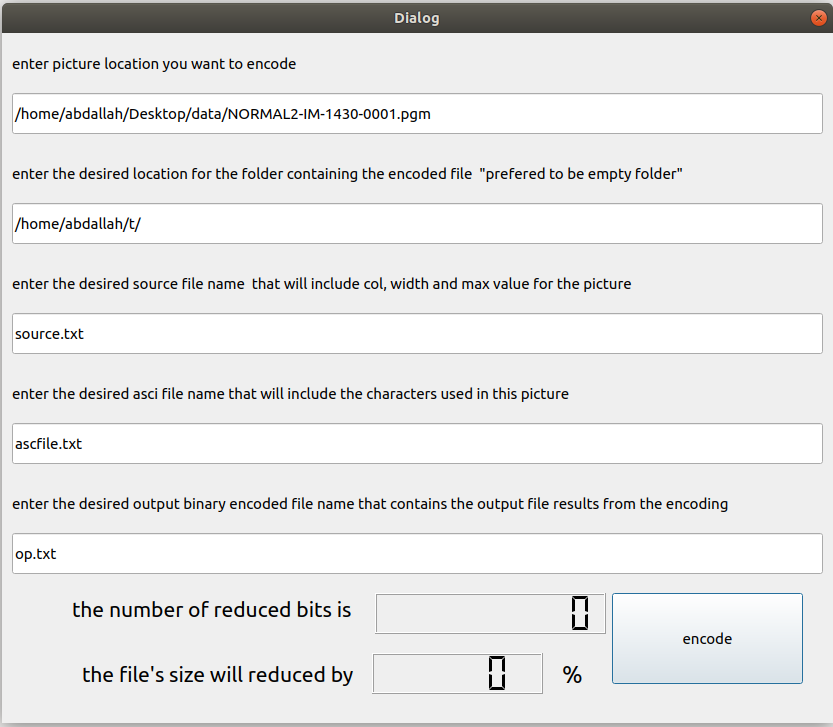
\includegraphics[width=0.8\linewidth]{figure 4}
\end{figure}\\
After you finish typing, just click on encode button, the number of reduced bits and its percentage will appear on the lcds as follows.\\
\begin{figure}[ht]
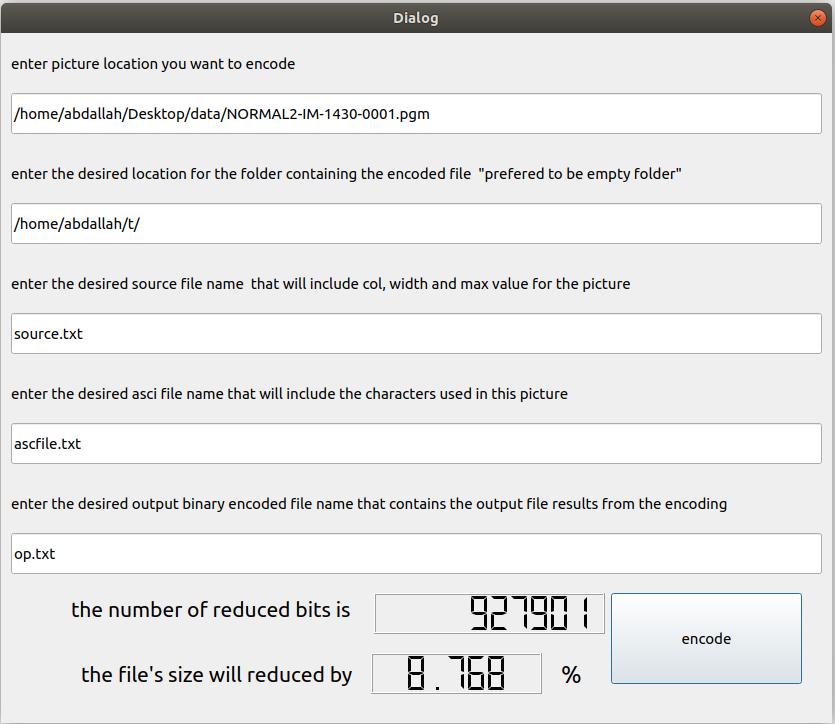
\includegraphics[width=0.8\linewidth]{figure 5}
\end{figure} \\
Now we have finished encoding, lets return back to our main page and click on decoding button, you will find similar inputs like for encoding.\\
1) we will enter the same folder we just made for encoding that will have now the encoded files.\\
2,3,4) enter the same  names you have chosen for these file in encoding.\\
5,6) enter also names for decoded file and picture.\\
\begin{figure}[ht]
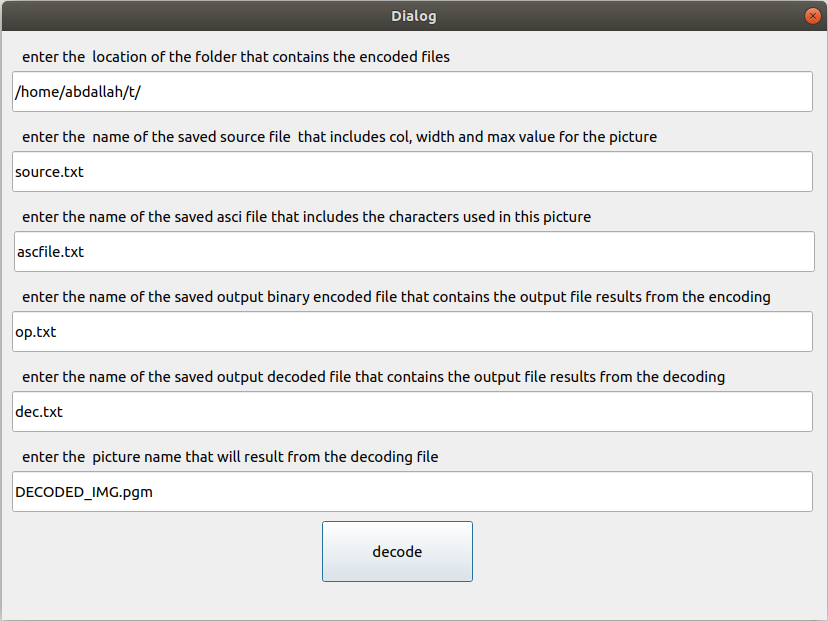
\includegraphics[width=0.8\linewidth]{figure 6}
\end{figure}\\
Now just press on decoding button and immediately a message we appear that decoding is finished.\\
\begin{figure}[ht]
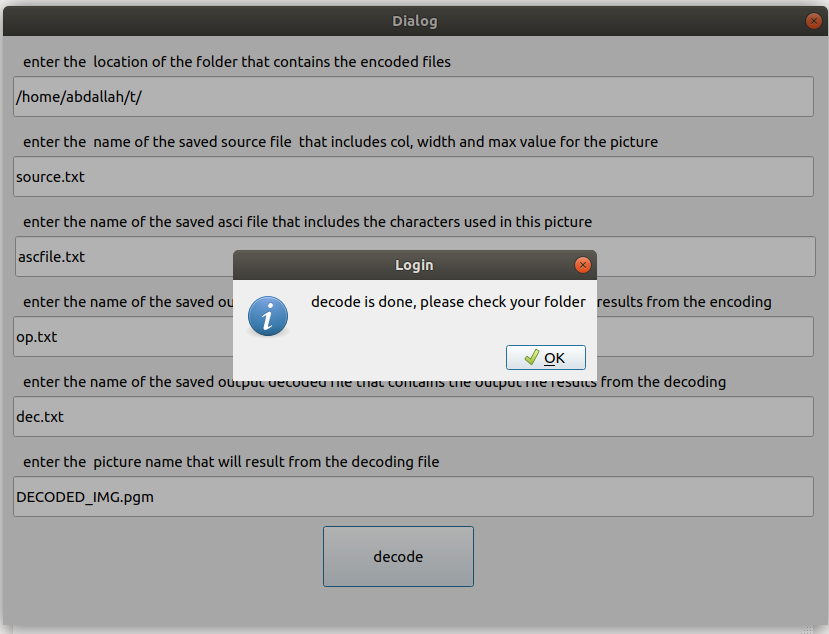
\includegraphics[width=0.8\linewidth]{figure 7}
\end{figure} \\
\newpage
That it, we finished, lets take a look on our empty folder, we will see that it contains 4 files and one picture, 3 file from encoding step, and the final file and the picture are from the decoding stage.\\
\begin{figure}[ht]
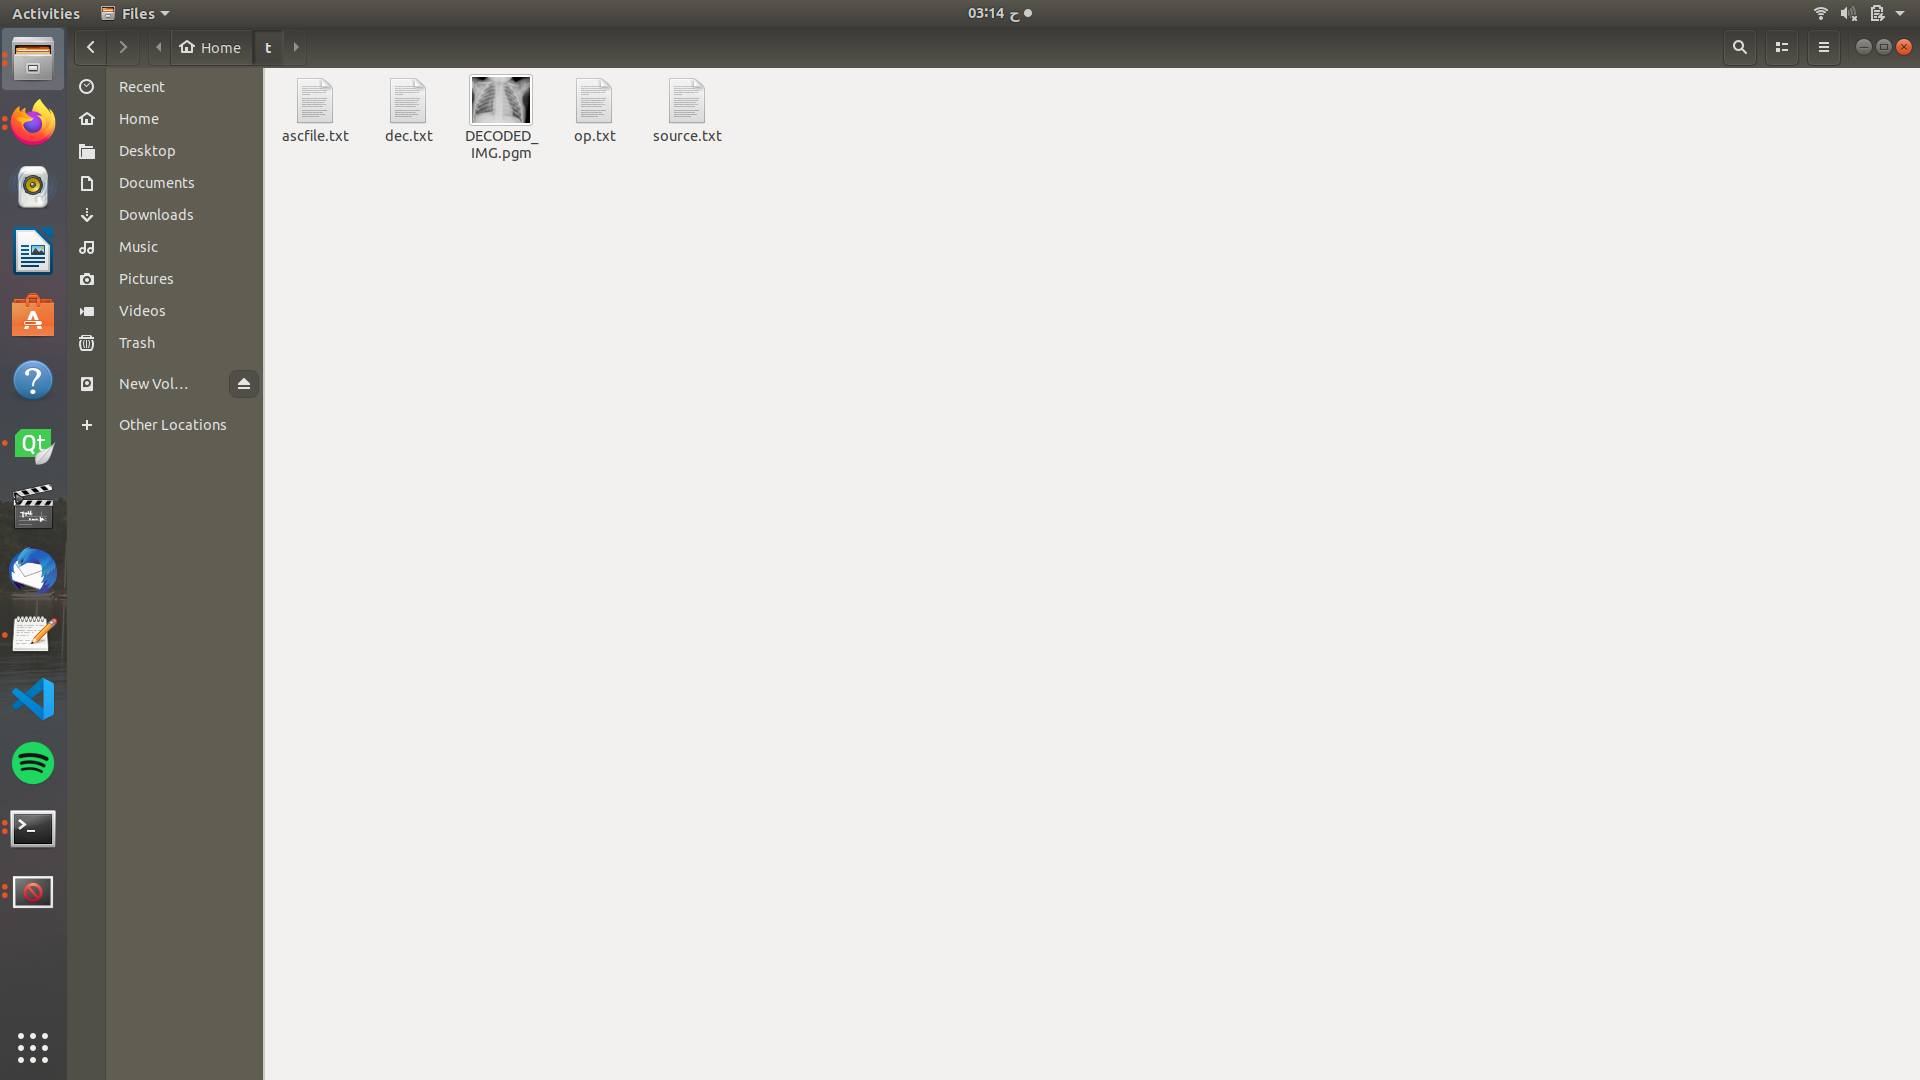
\includegraphics[width=0.8\linewidth]{figure 8}
\end{figure}\\
\newpage
Flow chart for the OUR GUI  that shows in few words our path from the beginning till the end.\\
\begin{figure}[ht]
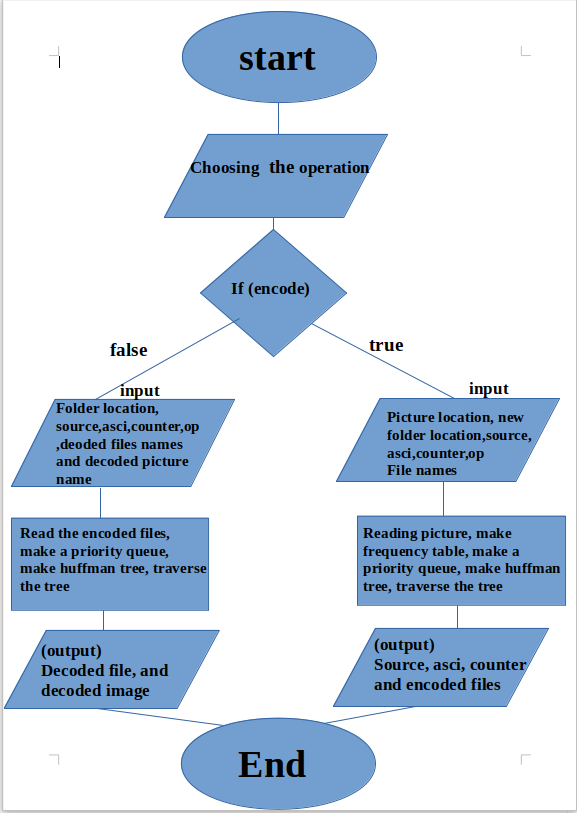
\includegraphics[width=0.8\linewidth]{figure 9}
\end{figure}\\
\newpage

\section{Contributions}
We need to say first that we didn’t make a clear tasks foe every one but we can say that in general each one of us has a major task so that he can help another team member and the rest of members could help him.\\
1) Abdallah Mohammad Shehata : for Huffman algorithm including encoding and decoding algorithms (build tree.h) file And report making.\\
2 ,3) Ezzeldeen esmail , Abdallah Tamer: making frequency table and sorting (frequency table.h) and report making\\
4) pola nagy : getting informations from the picture (pic-in.h)\\
5) youssef samir : determining the operation and some decoding codes and reading binary encoded file and asci and counter one (main.cpp)\\


\bibliography{bibliography.bib}
\bibliographystyle{ieeetr}



\end{document}
